\documentclass[10pt]{beamer}
%
% Choose how your presentation looks.
%
% For more themes, color themes and font themes, see:
% http://deic.uab.es/~iblanes/beamer_gallery/index_by_theme.html
%
\mode<presentation>
{
  \usetheme{default}      % or try Darmstadt, Madrid, Warsaw, ...
  \usecolortheme{default} % or try albatross, beaver, crane, ...
  \usefonttheme{default}  % or try serif, structurebold, ...
  \setbeamertemplate{navigation symbols}{}
  \setbeamertemplate{caption}[numbered]
} 

\usepackage[english]{babel}
\usepackage[utf8]{inputenc}
\usepackage[T1]{fontenc}

\title[Your Short Title]{Algebraic Filtering of Surfaces from 3D Medical Images with Julia}
\author{Alberto Paoluzzi, Miroslav Jirik}
\institute{Roma Tre University, Charles University}
\date{CAD 2020}

\usetheme{CambridgeUS}

\makeatletter
    \newenvironment{withoutheadline}{
        \setbeamertemplate{headline}[default]
        \def\beamer@entrycode{\vspace*{-\headheight}}
    }{}
\makeatother
\def\E{\mathbb{E}}

\begin{document}

\begin{frame}
  \titlepage
\end{frame}

% Uncomment these lines for an automatically generated outline.
%\begin{frame}{Outline}
%  \tableofcontents
%\end{frame}



\section{Introduction}
\begin{frame}{Geometric and topological computing}
\protect\hypertarget{geometric-and-topological-computing}{}

\framesubtitle{rethinking some foundations}

\begin{columns}[T]
\begin{column}{0.48\textwidth}
Complexity of geometric information stems from dramatic increase in
\emph{size}, \emph{diversity}, and \emph{complexity} of
\textbf{geometric data}:

\begin{itemize}
\tightlist
\item
  point clouds,
\item
  boundary meshes,
\item
  NURBs representations,
\item
  finite element meshes,
\item
  CT scans,
\item
  and so on
\end{itemize}
\end{column}

\begin{column}{0.48\textwidth}
Emerging applications (e.g. \textbf{medical 3D}) require the
\textbf{convergence of data structures} from:

\begin{itemize}
\tightlist
\item
  3d computer imaging
\item
  computer graphics
\item
  solid modeling
\item
  computer-aided geometric design
\item
  discrete meshing of domains
\item
  physical simulations
\end{itemize}
\end{column}
\end{columns}

The goals of \emph{unification}, \emph{scalability}, and
\emph{distributed computing} call for \emph{rethinking some foundations}
of geometric and topological computing

\end{frame}

\begin{frame}{Motivation for a new start}
\protect\hypertarget{motivation-for-a-new-start}{}

\begin{columns}[T]
\begin{column}{0.48\textwidth}
\begin{block}{Quad-edge data structure \cite{Guibas1985}}

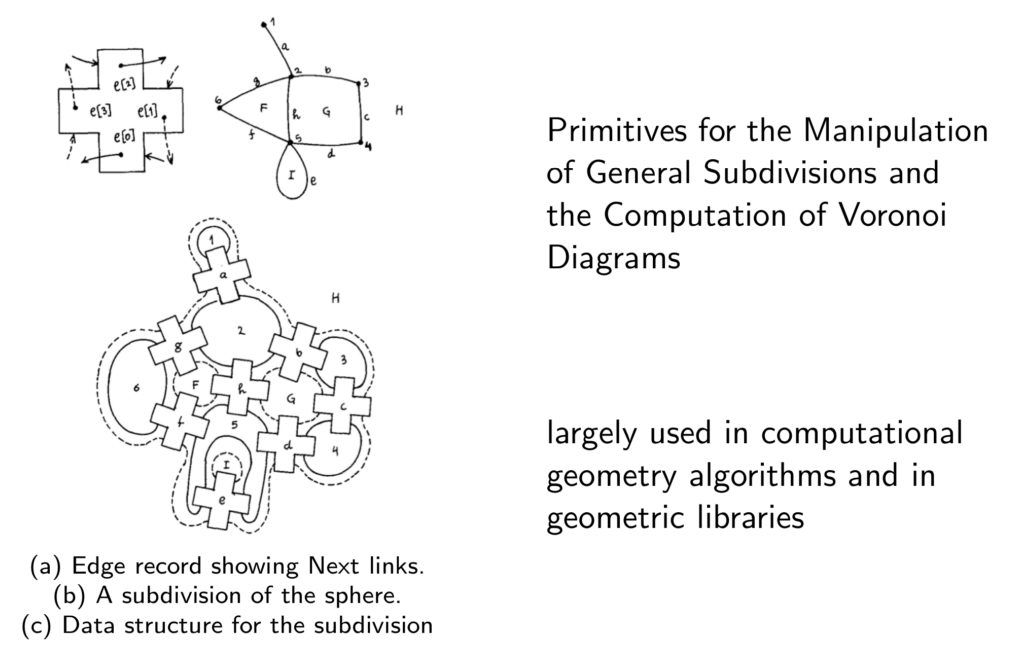
\includegraphics{figs/Guibas1985_quad_edge.png}~

\end{block}

\begin{block}{Hybrid Edge data sturcture \cite{Kalay1989}}

a topological data structure for vertically integrated geometric
modelling

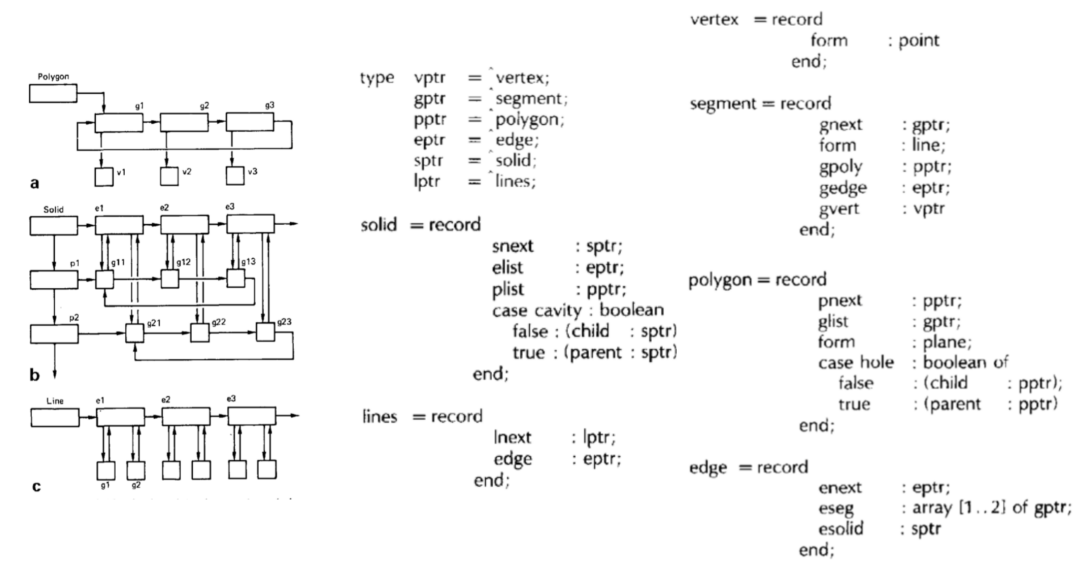
\includegraphics{figs/Kalay1989_hybrid_edge.png}~

\end{block}
\end{column}

\begin{column}{0.48\textwidth}
\begin{block}{Partial-Entity data structure \cite{SangHunLee2001}}

Compact Non-Manifold Boundary Representation Based on Partial
Topological Entities
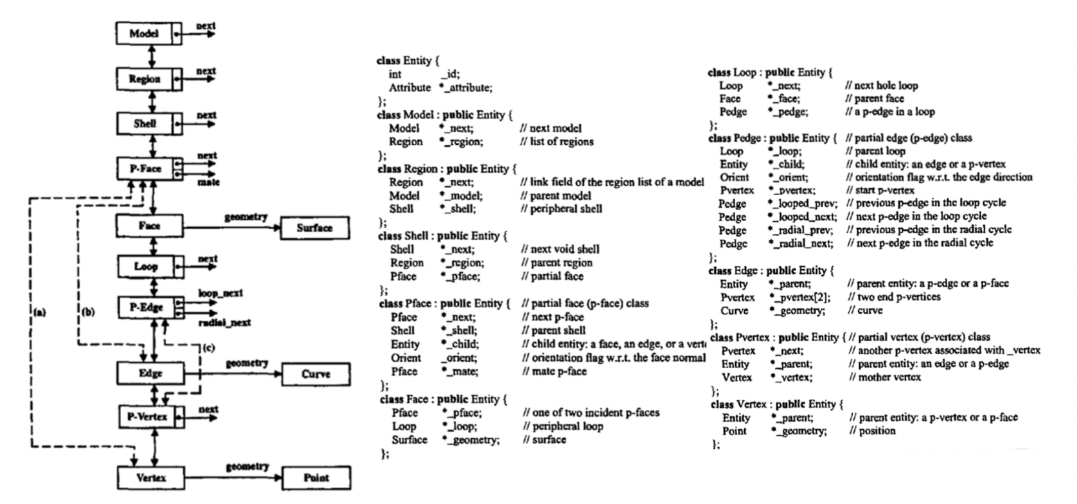
\includegraphics{figs/SangHunLee2001_partial_entity.png}~

\end{block}

\begin{block}{Coupling Entities data structure
\cite{yamaguchi1995nonmanifold}}

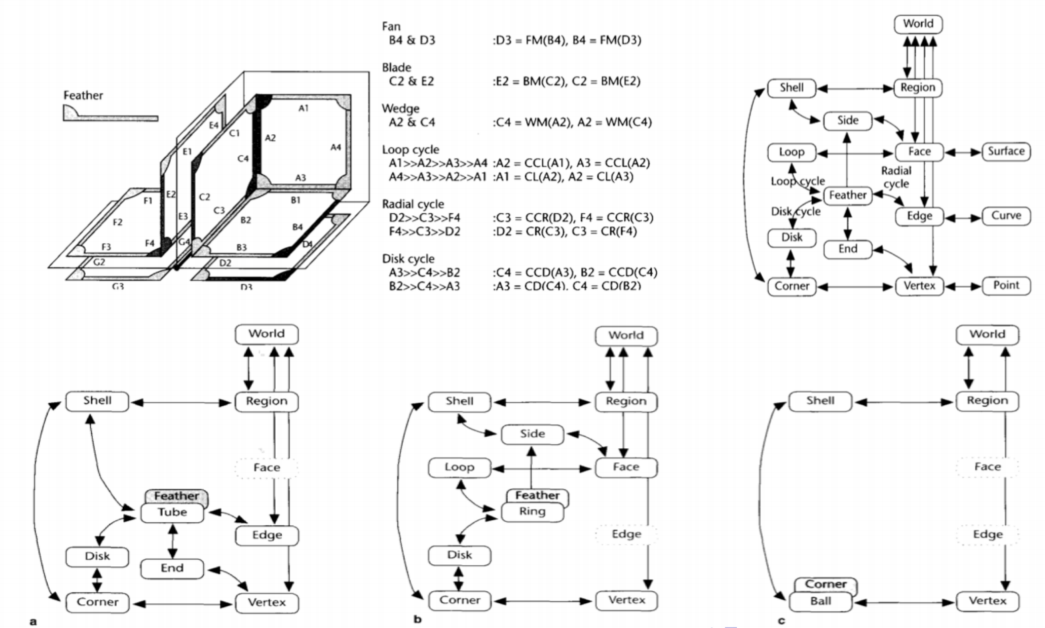
\includegraphics{figs/yamaguchi1995nonmanifold.png}~

\end{block}
\end{column}
\end{columns}

\begin{block}{first sub}

\begin{itemize}
\tightlist
\item
  asdf
\item
  neks
\end{itemize}

\end{block}

\begin{block}{second sub}

\begin{itemize}
\tightlist
\item
  asf
\item
  woens
\end{itemize}

\end{block}

\end{frame}

\begin{frame}{third slide}
\protect\hypertarget{third-slide}{}

asdfa sd asd fas

\end{frame}

\begin{frame}{My slide}
\protect\hypertarget{my-slide}{}

\begin{block}{First column}

contents

\end{block}

\begin{block}{Second column}

contents

\end{block}

\end{frame}



\begin{frame}{}
\vfill
\centering

\begin{beamercolorbox}[sep=8pt,center,shadow=true,rounded=true]{title}
    Linear Algebraic Reperesentation
\end{beamercolorbox}
\vfill
    
    % \begin{block}{}
    % \end{block}
\end{frame}


\begin{frame}{Linear Alebraic Representation (LAR)}
LAR introduced in~\cite{Dicarlo:2014:TNL:2543138.2543294}, aims to represent the \emph{chain complex}~\cite{DiCarlo2009,TSAS} generated by a piecewise-linear \emph{geometric complex} embedded either in 2D or in 3D. 
This representation provides a minimal characterization of geometry and topology of a cellular complex, through 
\begin{enumerate}
    \item[a)] the embedding mapping 
        $\mu : C_0 \to \E^d$ of 0-cells (vertices)
    \item[b)] a description of $d$-cells and/or $(d-1)$-cells as subsets of vertices. 
\end{enumerate}


When evaluated, it is able to return the whole chain complex:
\begin{equation}
C_\bullet = (C_p, \partial_p) := 
C_3 
\substack{
\delta_2 \\
\longleftarrow \\
\longrightarrow \\
\partial_3 
}
C_2 
\substack{
\delta_1 \\
\longleftarrow \\
\longrightarrow \\
\partial_2 
}
C_1  
\substack{
\delta_0 \\
\longleftarrow  \\
\longrightarrow \\
\partial_1 
}
C_0 .
\end{equation}


i.e., the whole sequence of graded linear \emph{chain spaces} $C_p$, and any linear \emph{boundary} $\partial_p$ and \emph{coboundary} $\delta_p$ map, with $\delta_p=\partial_{p-1}^\top$ between them.
 The \emph{domain} of \textsc{lar} is the set of \textbf{chain complexes} generated by cell $d$-complexes ($2\leq d\leq 3$). The computer \emph{representations} of \textsc{lar} are \textbf{sparse binary matrices} to represent both the operators and the bases of chain spaces. Note that in algebraic topology a $p$-chain is defined as a linear combination of $p$-cells with scalars from a field. 
 
%  When the scalar coefficients are from $\{-1, 0, +1\}$, a chain may represent \emph{any (oriented) subset of cells} from the cellular complex.
% Scalars from $\{0, 1\}$ are used for non-oriented complexes.

% \begin{columns}
% \end{columns}
% \begin{figure}
%     \centering
%     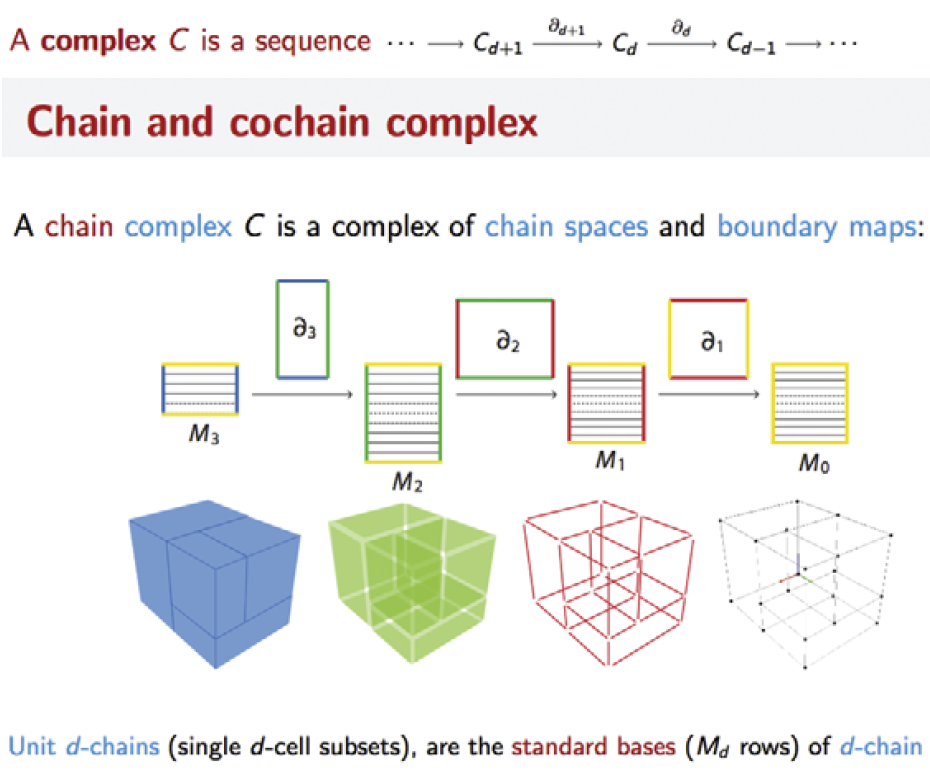
\includegraphics[width=0.95\textwidth]{figs/L02-chain-complex.png}
%     % \caption{Caption}
%     % \label{fig:my_label}
% \end{figure}
    
\end{frame}




\begin{frame}
\begin{figure}
    \centering
    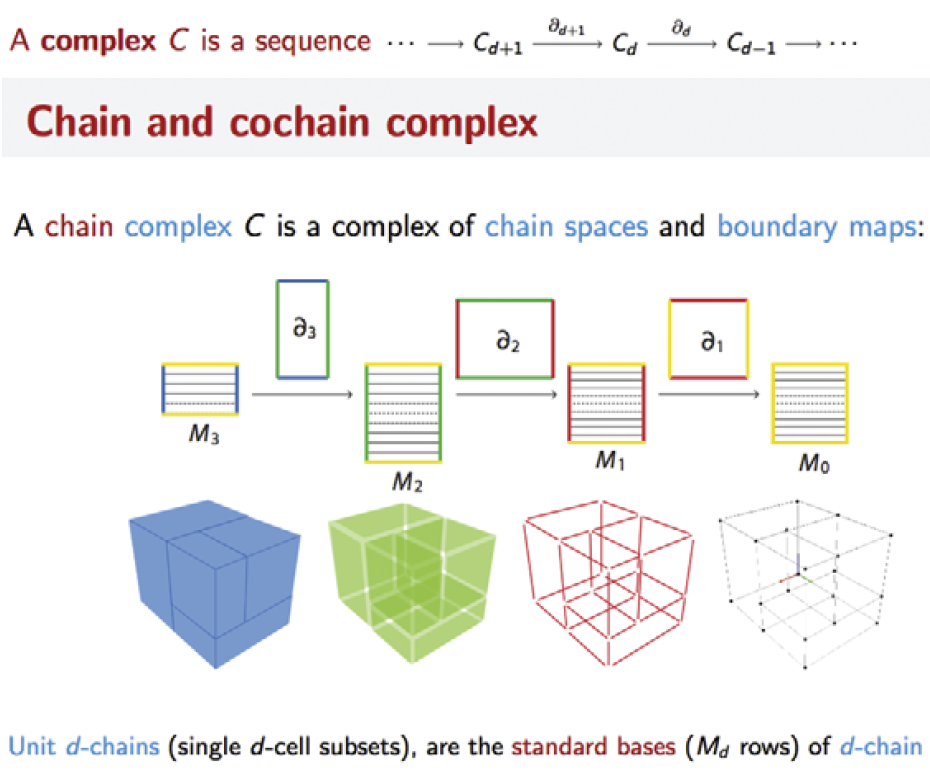
\includegraphics[width=0.95\textwidth]{figs/L02-chain-complex.png}
    % \caption{Caption}
    % \label{fig:my_label}
\end{figure}
    
\end{frame}


\begin{frame}
\begin{figure}
    \centering
    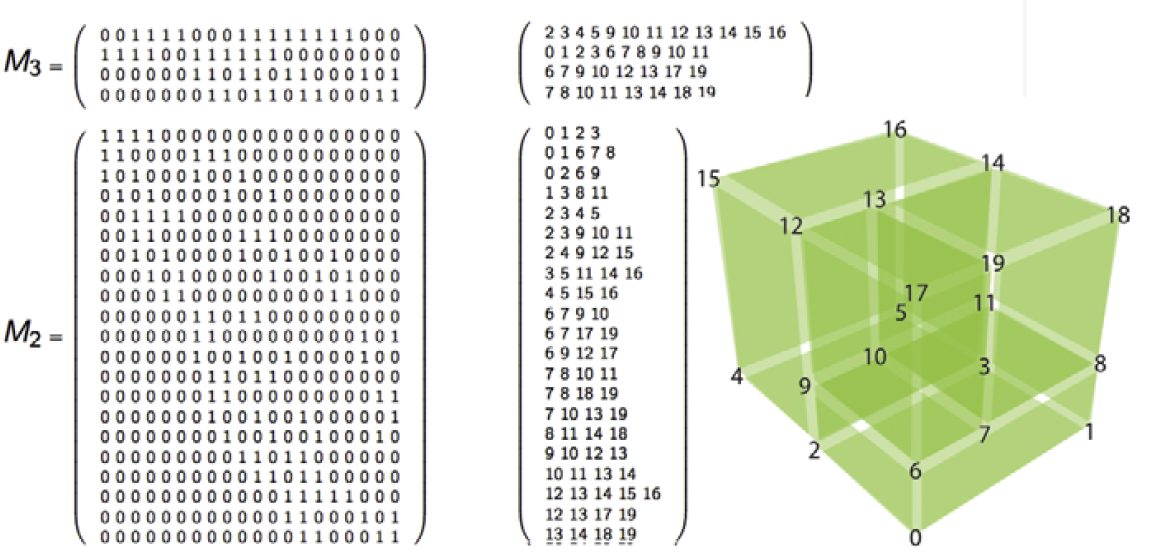
\includegraphics[width=\textwidth]{figs/L02-characteristic-matrices.png}
    % \caption{Caption}
    % \label{fig:my_label}
\end{figure}
\end{frame}

\begin{frame}{Construction of boundary matrix $\partial_d$}

Here we discuss a surface extraction based on basic algebraic topology and linear algebra, using linear spaces $C_p$ of chains (of cells) of dimension $0 \leq p \leq 3$ and the boundary matrix $[\partial_3] : C_3 \to C_2$.
    
\[
[\partial_p](i,j)=1\quad\mbox{if}\quad n_{i,j} = \sum_{k} m_{i,k}m_{k,j}=\texttt{\#}c^i_{p-1} \quad\mbox{and}\quad [\partial_p](i,j)=0 \quad\mbox{otherwise}.  
\]

% Look for this purpose at the rows of matrix $[\partial_3]^t$ in Figure~\ref{fig:boundary_matrix_4x4x4}, where 

   The binary image of \emph{sparse} coboundary matrix  $\left[\delta_2\right] = \left[\partial_3\right]^t : C_2 \to C_3$,
   built for a small volumetric data (or a brick) with shape $(4,4,4)$. 
%   Note that the number of rows equates the size $4\times 4\times 4 = 64$ of the voxel set; the number of columns is $d\,n\,(1+n)^{d-1} = 3\times 4\times 25 = 300$. Of course, the number of non-zeros per row (cardinality of the facet set of a single voxel) is six, whereas the number of non-zeros per column is generally two, but on boundary facets. 
   
   The letter F stands for \emph{Faces}, on matrix columns, and the C stands for \emph{Cells} (3-cells) on matrix rows.

% the matrix is  transposed for better shape ratio.
% The unit incidence coefficients in $\left[\partial_3\right]$, shown as white pixels, are accordingly located by filtering the $n_{i,j}$ elements with value 4. All the other matrix element are set to 0, shown as black pixels. 
\begin{center}
  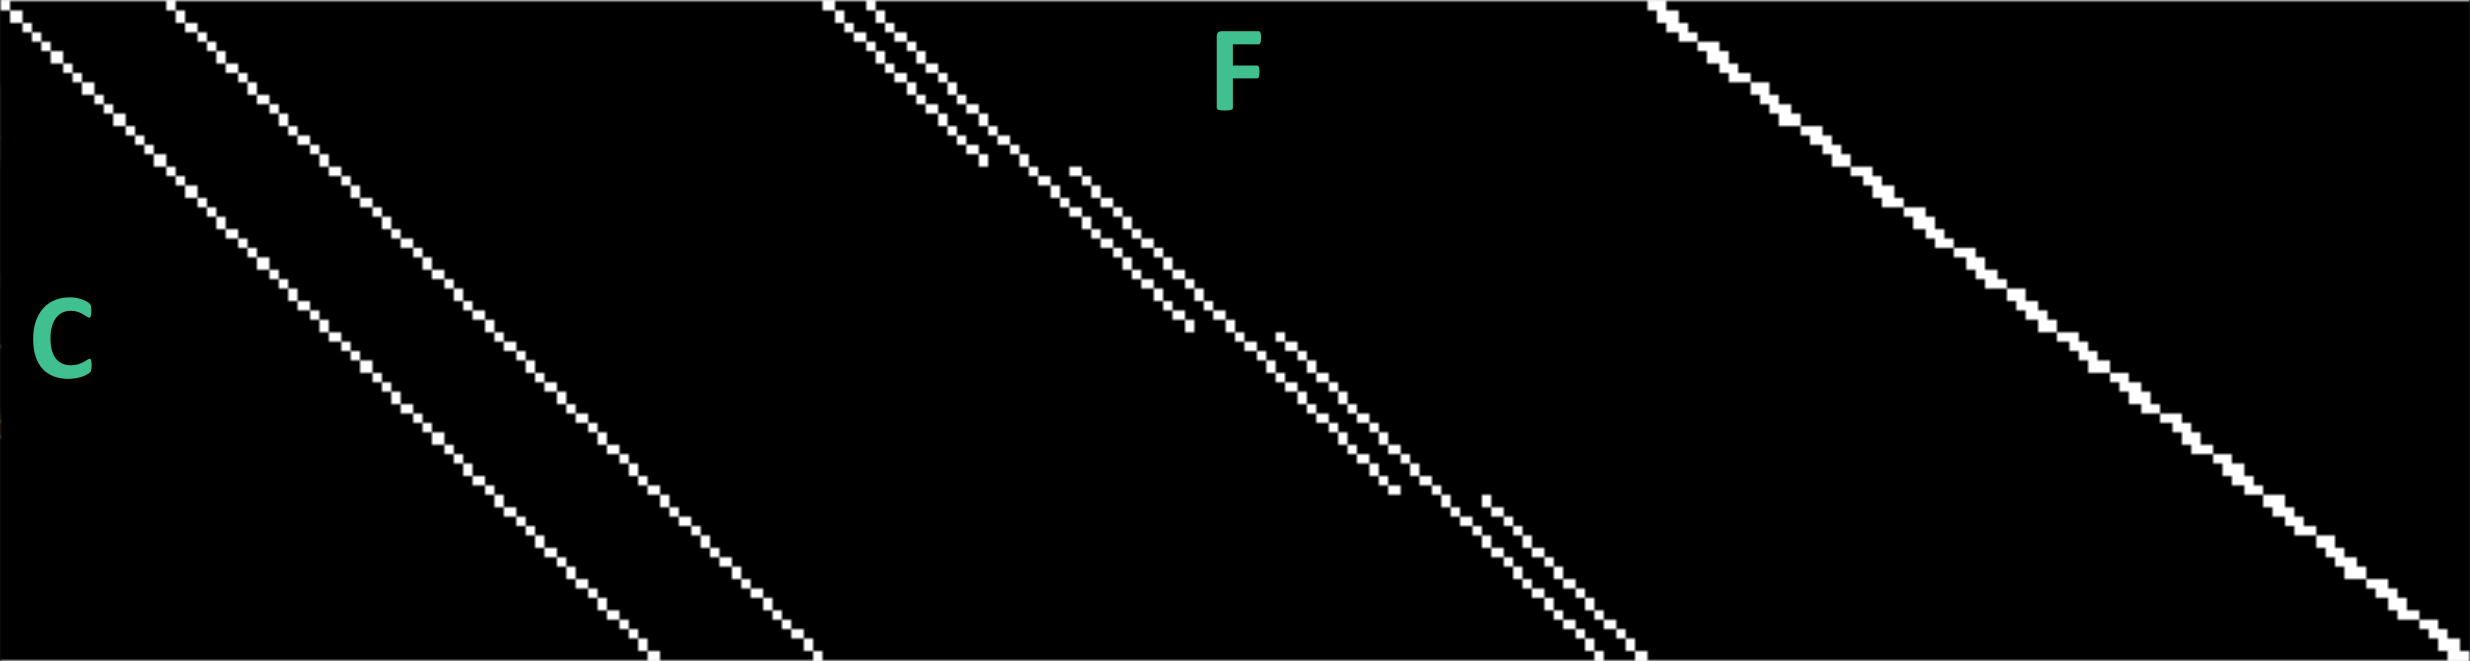
\includegraphics[width=0.75\linewidth]{figs/boundary_matrix_4x4x4_desc.png} 
\end{center}
  
%   \caption{

\end{frame}


\begin{frame}{Lar-surf}
\begin{figure}
    \centering
            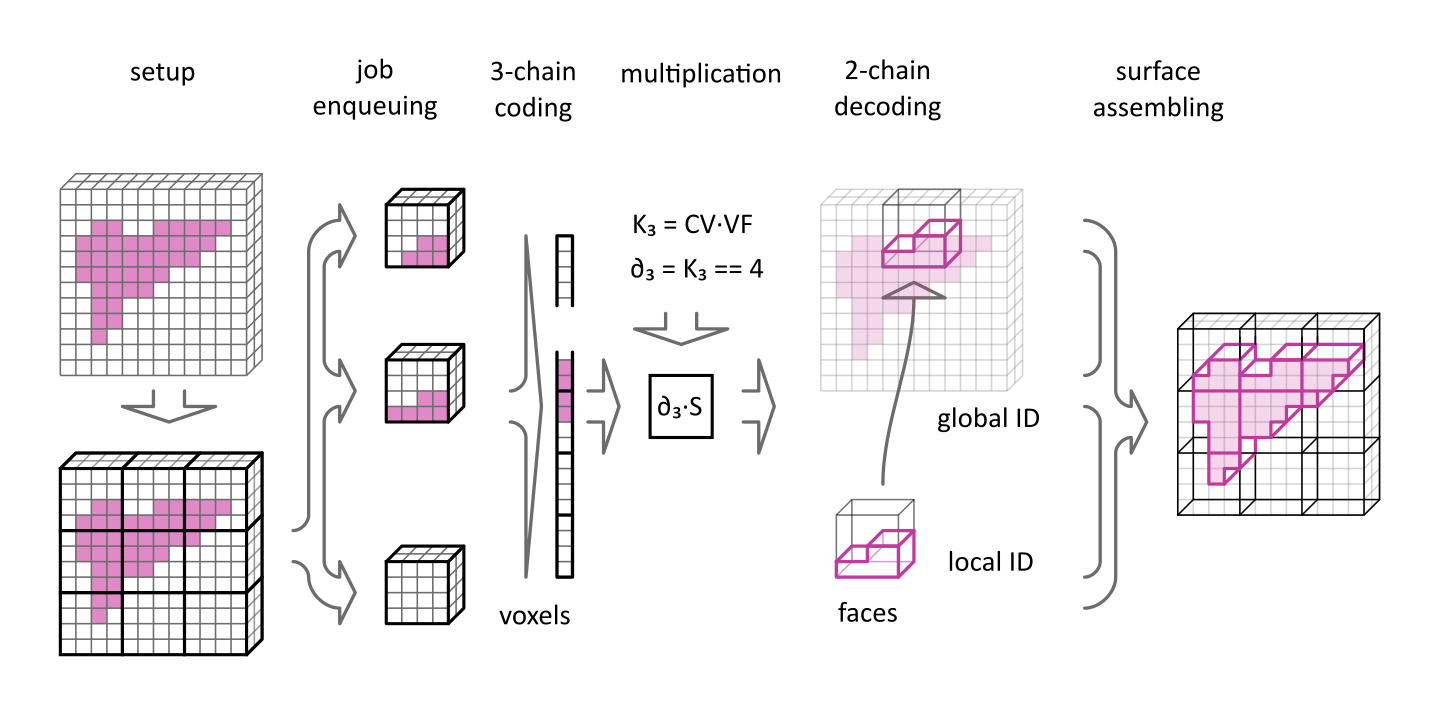
\includegraphics[width=\textwidth]{figs/schema_horizontal.png}
    \caption{LAR surface extraction scheme}
\end{figure}
    
\end{frame}

\begin{frame}{Surface representation with LAR}
\begin{figure}
    \centering
            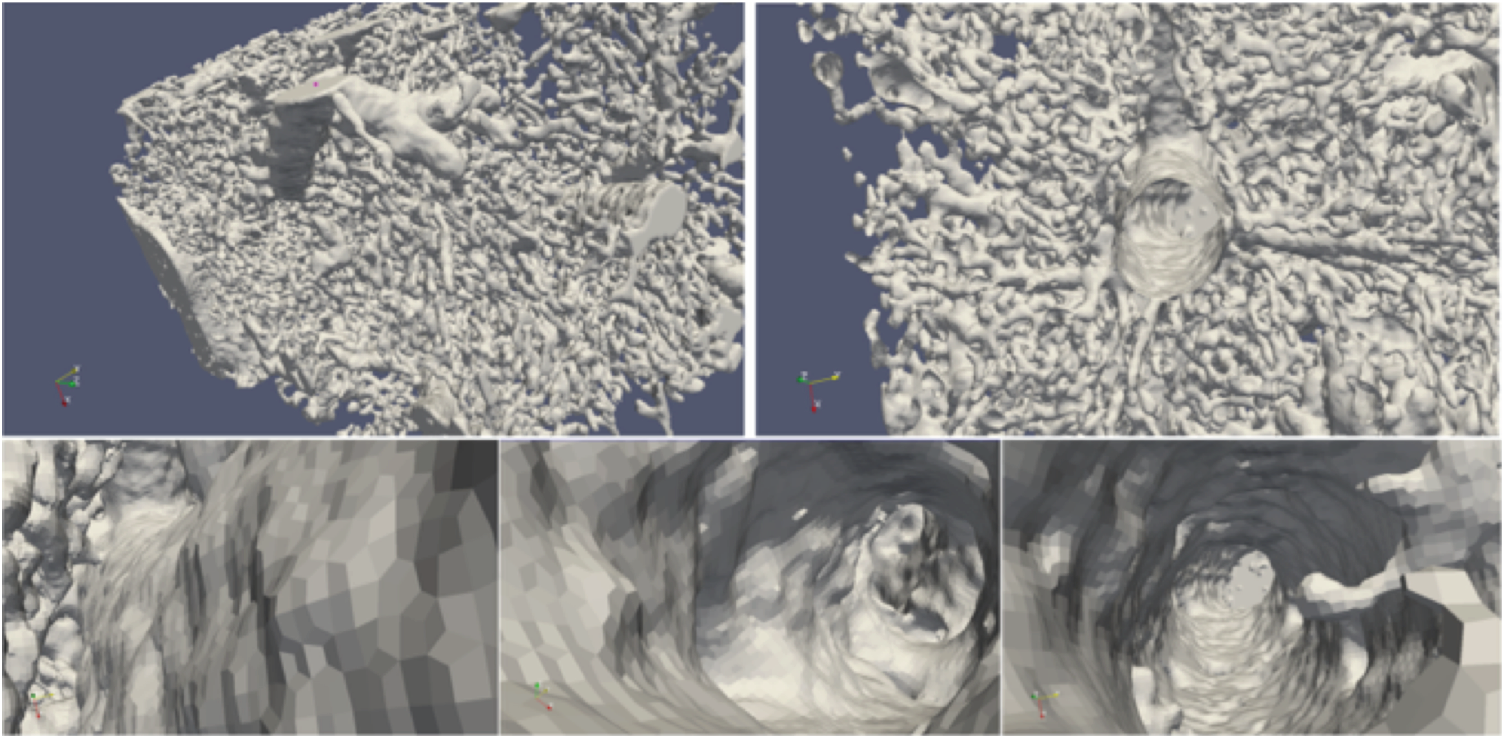
\includegraphics[width=\textwidth]{figs/paoluzzi_dicarlo_furiani_jirik_2016.png}
    \caption{Liver microstructure\cite{Paoluzzi2016}}
\end{figure}
    
\end{frame}


\begin{frame}{Surface extraction with LAR}
\begin{figure}
    \centering
            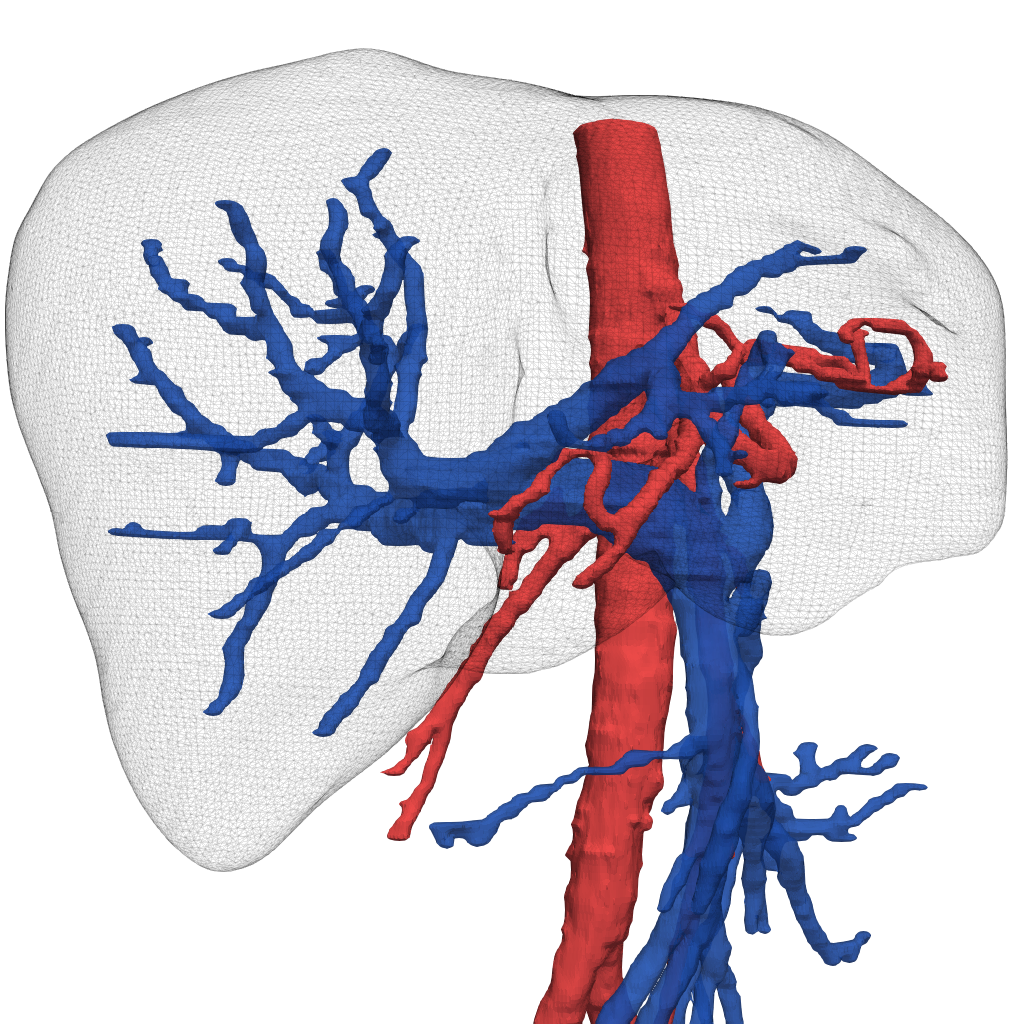
\includegraphics[width=0.6\textwidth]{figs/ircad01_liver_tricolore_01.png}
\end{figure}
    
\end{frame}



\begin{frame}{Introduction}

\begin{itemize}
  \item Your introduction goes here!
  \item Use \texttt{itemize} to organize your main points.
\end{itemize}

\vskip 1cm

\begin{block}{Examples}
Some examples of commonly used commands and features are included, to help you get started.
\end{block}

\end{frame}

\section{Some \LaTeX{} Examples}

\subsection{Tables and Figures}

\begin{frame}{Tables and Figures}

\begin{itemize}
\item Use \texttt{tabular} for basic tables --- see Table~\ref{tab:widgets}, for example.
\item You can upload a figure (JPEG, PNG or PDF) using the files menu. 
\item To include it in your document, use the \texttt{includegraphics} command (see the comment below in the source code).
\end{itemize}

% Commands to include a figure:
%\begin{figure}
%\includegraphics[width=\textwidth]{your-figure's-file-name}
%\caption{\label{fig:your-figure}Caption goes here.}
%\end{figure}

\begin{table}
\centering
\begin{tabular}{l|r}
Item & Quantity \\\hline
Widgets & 42 \\
Gadgets & 13
\end{tabular}
\caption{\label{tab:widgets}An example table.}
\end{table}

\end{frame}

\subsection{Mathematics}

\begin{frame}{Readable Mathematics}

Let $X_1, X_2, \ldots, X_n$ be a sequence of independent and identically distributed random variables with $\text{E}[X_i] = \mu$ and $\text{Var}[X_i] = \sigma^2 < \infty$, and let
\[ S_n = \frac{X_1 + X_2 + \cdots + X_n}{n}
      = \frac{1}{n}\sum_{i}^{n} X_i \]
denote their mean. Then as $n$ approaches infinity, the random variables $\sqrt{n}(S_n - \mu)$ converge in distribution to a normal $\mathcal{N}(0, \sigma^2)$.

\end{frame}

\begin{frame}[t,allowframebreaks]
\frametitle{References}
\bibliographystyle{alpha}
\bibliography{references.bib,TSAS-2019.bib}
\end{frame}

\end{document}
